% !TeX program = lualatex
% Lualatex is important to render Fira fonts; with pdflatex it's just the regular one
\documentclass[12pt]{beamer}


\usepackage{xcolor}

\usetheme{metropolis}
\usepackage{appendixnumberbeamer}

% adjust the background to be completely white
\setbeamercolor{background canvas}{bg=white}

\usepackage{booktabs}
\usepackage[scale=2]{ccicons}

\usepackage{pgfplots}
\usepgfplotslibrary{dateplot}

% typeset mathematics on serif
\usefonttheme[onlymath]{serif}

% better bibliography using biber as backend
\usepackage[natbib=true,backend=biber,style=authoryear-icomp,maxbibnames=30,maxcitenames=3,uniquelist=false,giveninits=true,doi=false,url=true,dashed=false,isbn=false]{biblatex}
% shared bibliogrphy
\addbibresource{../dl4nlp-bibliography.bib}
% disable "ibid" for repeated citations
\boolfalse{citetracker}

% TODOs
\usepackage{todonotes}
\let\todox\todo
\renewcommand\todo[1]{\todox[inline]{#1}}

\definecolor{76abdf}{RGB}{118, 171, 223}

\setbeamercolor{frametitle}{bg=76abdf, fg=white}

\usepackage{xspace}
\newcommand{\themename}{\textbf{\textsc{metropolis}}\xspace}

% POS tags
\newcommand*\POS[1]{\textsubscript{\texttt{#1}}} % tag with part of speech

% parse tree
\usepackage{qtree}

% NNEts
\usepackage{tikz}
\usetikzlibrary{matrix}
\usetikzlibrary{positioning}
\usetikzlibrary{calc}
\usetikzlibrary{backgrounds}
\usetikzlibrary{fit} % for hightligting by calling "fit"


% for derivatives, https://tex.stackexchange.com/a/412442
\usepackage{physics}

% code listing
\usepackage{listings}

% XML formatting; taken from https://gist.github.com/sebald/3130827
\definecolor{dkgreen}{rgb}{0,0.6,0}
\definecolor{gray}{rgb}{0.5,0.5,0.5}
\definecolor{mauve}{rgb}{0.58,0,0.82}
\definecolor{gray}{rgb}{0.4,0.4,0.4}
\definecolor{darkblue}{rgb}{0.0,0.0,0.6}
\definecolor{lightblue}{rgb}{0.0,0.0,0.9}
\definecolor{cyan}{rgb}{0.0,0.6,0.6}
\definecolor{darkred}{rgb}{0.6,0.0,0.0}
\lstset{
	basicstyle=\ttfamily\scriptsize,
	columns=fullflexible,
	showstringspaces=false,
	numbers=left,                   % where to put the line-numbers
	numberstyle=\tiny\color{gray},  % the style that is used for the line-numbers
	stepnumber=1,
	numbersep=5pt,                  % how far the line-numbers are from the code
	backgroundcolor=\color{white},      % choose the background color. You must add \usepackage{color}
	showspaces=false,               % show spaces adding particular underscores
	showstringspaces=false,         % underline spaces within strings
	showtabs=false,                 % show tabs within strings adding particular underscores
	frame=none,                   % adds a frame around the code
	rulecolor=\color{black},        % if not set, the frame-color may be changed on line-breaks within not-black text (e.g. commens (green here))
	tabsize=2,                      % sets default tabsize to 2 spaces
	captionpos=b,                   % sets the caption-position to bottom
	breaklines=true,                % sets automatic line breaking
	breakatwhitespace=false,        % sets if automatic breaks should only happen at whitespace
	title=\lstname,                   % show the filename of files included with \lstinputlisting;
	% also try caption instead of title  
	commentstyle=\color{gray}\upshape
}
\lstdefinelanguage{XML}
{
	morestring=[s][\color{mauve}]{"}{"},
	morestring=[s][\color{black}]{>}{<},
	morecomment=[s]{<?}{?>},
	morecomment=[s][\color{dkgreen}]{<!--}{-->},
	stringstyle=\color{black},
	identifierstyle=\color{lightblue},
	keywordstyle=\color{red},
	morekeywords={xmlns,xsi,noNamespaceSchemaLocation,type,id,x,y,source,target,version,tool,transRef,roleRef,objective,eventually}% list your attributes here
}


% tables with color
\usepackage{colortbl}


\title{Deep Learning for Natural Language Processing}
\subtitle{Lecture 6 -- Convolutional Neural Networks}
\date{May 18, 2021}
\author{Dr.\ Ivan Habernal}
\institute{Trustworthy Human Language Technologies  \hfill 
\includegraphics[height=.8cm]{img/logo-trusthlt.pdf} \\
Department of Computer Science\\
Technical University of Darmstadt \hfill \texttt{www.trusthlt.org}}
%\titlegraphic{\hfill }

\begin{document}

\maketitle


%\begin{frame}{Table of contents}
%  \setbeamertemplate{section in toc}[sections numbered]
%  \tableofcontents[hideallsubsections]
%\end{frame}

%\section{Administrative course issues}

\begin{frame}{This lecture}
	
Today: Classifying sentences or documents

\end{frame}


\begin{frame}{Motivation example}
	


Predicting the sentiment (positive, negative, or neutral)\footnote{\url{https://www.rottentomatoes.com}}

\begin{columns}
	\begin{column}{4cm}
\begin{figure}
	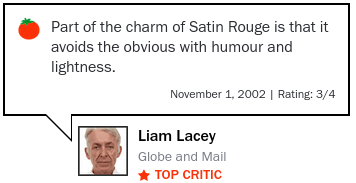
\includegraphics[width=\linewidth]{img/review1.png}
\end{figure}
	\end{column}
\begin{column}{7cm}
\begin{figure}
	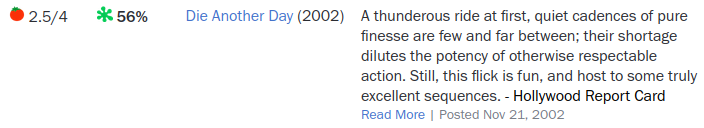
\includegraphics[trim={6cm 0 0 0},clip,width=\linewidth]{img/review2.png}
\end{figure}

\end{column}
\end{columns}
	


- Some of the words are \textbf{very informative} of the sentiment (charm, fun, excellent) other
words are less informative (Still, host, flick, lightness, obvious, avoids)


- Informative clue is informative regardless of its position in the sentence

	
\end{frame}


\begin{frame}{Motivation}

Problem 1: Variable-sized input

- standard MLP always expect the same input size



Problem 2: Relevance of words

- “to” and “a” are not very informative, but content words like “kidnapping” are important for most tasks independent of their position in the input


Problem 3: MLP may have too many parameters (“too complex models”) in certain situations 

\end{frame}


\begin{frame}{This lecture}
Convolution and pooling

Convolutional networks for NLP
\end{frame}

\iffalse
\begin{frame}{Idea of convolution}
“A convolutional neural network is designed to identify indicative local predictors in a large structure, and combine them to produce a fixed size vector representation of the structure, capturing these local aspects that are most informative for the prediction task at hand.“ 
	
Yoav Goldberg 

\end{frame}
\fi

\begin{frame}{1-D convolution operation}
	
	$$
	s[i] = (f * g) [i] = \sum_{m = -M}^{M} f[i - m] \cdot g[m]
	$$
	
	where
	
	\begin{itemize}
		\item $s[i]$ is the output at position $i$
		\item $f$ is the input representation
		\item $*$ is the convolution operator
		\item $i$ is the current position in input
		\item $M$ is the window size
		\item $g$ is the filter (kernel)
	\end{itemize}
	
	Beware of many different terminologies in the literature!
	
\end{frame}


\begin{frame}[fragile]{1-D convolution operation example}
	
	\usetikzlibrary{matrix}
\usetikzlibrary{positioning}
\usetikzlibrary{calc}
\usetikzlibrary{backgrounds}
\usetikzlibrary{fit} % for hightligting by calling "fit"

\tikzset{
	mtx/.style={
		matrix of math nodes,
		left delimiter={[}, right delimiter={]}
	},
	hlt/.style={opacity=0.1, line width=4 mm, line cap=round},
	hltr/.style={opacity=0.5, rounded corners=2pt, inner sep=-1pt}
}

\begin{tikzpicture}

\matrix[mtx, ampersand replacement=\&] (X) at (2,2) {
	1 \& 1 \& 1 \& 0 \& 0 \\ 
};

\matrix[mtx,  ampersand replacement=\&, right=5ex of X] (filterg) { 
	1 \& 0 \& 1 \\
};

\matrix[mtx, ampersand replacement=\&, nodes={anchor=west}, right=of filterg] (mu) {
	? \& ? \& ?  \\
};

%\draw[-stealth, color=red] (X-1-1.south west) -| (beta-6-1.south west);

\node at ($(X.east) !0.5! (filterg.west)$) {$*$};
\node at ($(filterg.east)!0.5!(mu.west)$) {$=$};%

\begin{scope}[every node/.style={align=center,text width=3cm}]
\node[below=0.2cm of X] (inputdsc) {\scriptsize Input representation $f$};
\node[below=0.2cm of filterg] (convdesc) {\scriptsize Filter $g$ \\ (also `kernel')};
\node[below=0.2cm of mu] (outdesc) {\scriptsize Convolved output};
\end{scope}


\end{tikzpicture}
	
\end{frame}

\begin{frame}{1-D convolution operation example}
	
	\usetikzlibrary{matrix}
\usetikzlibrary{positioning}
\usetikzlibrary{calc}
\usetikzlibrary{backgrounds}
\usetikzlibrary{fit} % for hightligting by calling "fit"

\tikzset{
	mtx/.style={
		matrix of math nodes,
		left delimiter={[}, right delimiter={]}
	},
	hlt/.style={opacity=0.1, line width=4 mm, line cap=round},
	hltr/.style={opacity=0.5, rounded corners=2pt, inner sep=-1pt}
}

\begin{tikzpicture}

\matrix[mtx, ampersand replacement=\&] (X) at (2,2) {
	1 \& 1 \& 1 \& 0 \& 0 \\ 
};

\matrix[mtx,  ampersand replacement=\&, right=5ex of X] (filterg) { 
	1 \& 0 \& 1 \\
};

\matrix[mtx, ampersand replacement=\&, nodes={anchor=west}, right=of filterg] (mu) {
	2 \& ? \& ?  \\
};

%\draw[-stealth, color=red] (X-1-1.south west) -| (beta-6-1.south west);

\node at ($(X.east) !0.5! (filterg.west)$) {$*$};
\node at ($(filterg.east)!0.5!(mu.west)$) {$=$};%


\begin{scope}[on background layer]
%\node[hltr, fill=gray, fit=(beta-1-1)] {};
%\node[hltr, fill=red, fit=(beta-2-1)(beta-3-1)] {};
%\node[hltr, fill=green, fit=(beta-4-1)(beta-6-1)] {};
%\node[hltr, fill=gray, fit=(X-1-1)(X-12-1)] {};
\node[hltr, fill=orange, fit=(filterg-1-1)(filterg-1-3)] {};
\node[hltr, fill=orange, fit=(X-1-1)(X-1-3)] {};
\node[hltr, fill=orange, fit=(mu-1-1)(mu-1-1)] {};
%\node[hltr, fill=green, fit=(X-1-4)(X-12-6)] {};
\end{scope}

\draw[->, lightgray, thick] (filterg-1-1) to[out = 90, in = 90] (X-1-1);

\begin{scope}[every node/.style={align=center,text width=3cm}]
\node[below=0.2cm of X] (inputdsc) {\scriptsize Input representation $f$};
\node[below=0.2cm of filterg] (convdesc) {\scriptsize Filter $g$};
\node[below=0.2cm of mu] (outdesc) {\scriptsize Convolved output};
%\node[above=0cm of hidden] (hiddendsc) {\scriptsize Hidden layer};
%\node[above=0cm of output] (outputdsc) {\scriptsize Output};
\end{scope}


\end{tikzpicture}
	
	\usetikzlibrary{matrix}
\usetikzlibrary{positioning}
\usetikzlibrary{calc}
\usetikzlibrary{backgrounds}
\usetikzlibrary{fit} % for hightligting by calling "fit"

\tikzset{
	mtx/.style={
		matrix of math nodes,
		left delimiter={[}, right delimiter={]}
	},
	hlt/.style={opacity=0.1, line width=4 mm, line cap=round},
	hltr/.style={opacity=0.5, rounded corners=2pt, inner sep=-1pt}
}

\begin{tikzpicture}

\matrix[mtx, ampersand replacement=\&] (X) at (2,2) {
	1 \& 1 \& 1 \& 0 \& 0 \\ 
};

\matrix[mtx,  ampersand replacement=\&, right=5ex of X] (filterg) { 
	1 \& 0 \& 1 \\
};

\matrix[mtx, ampersand replacement=\&, nodes={anchor=west}, right=of filterg] (mu) {
	2 \& 1 \& ?  \\
};

%\draw[-stealth, color=red] (X-1-1.south west) -| (beta-6-1.south west);

\node at ($(X.east) !0.5! (filterg.west)$) {$*$};
\node at ($(filterg.east)!0.5!(mu.west)$) {$=$};%


\begin{scope}[on background layer]
\node[hltr, fill=orange, fit=(filterg-1-1)(filterg-1-3)] {};
\node[hltr, fill=orange, fit=(X-1-2)(X-1-4)] {};
\node[hltr, fill=orange, fit=(mu-1-2)(mu-1-2)] {};
\end{scope}

\draw[->, lightgray, thick] (filterg-1-1) to[out = 90, in = 90] (X-1-2);

\begin{scope}[every node/.style={align=center,text width=3cm}]
\node[below=0.2cm of X] (inputdsc) {\scriptsize Input representation $f$};
\node[below=0.2cm of filterg] (convdesc) {\scriptsize Filter $g$};
\node[below=0.2cm of mu] (outdesc) {\scriptsize Convolved output};
%\node[above=0cm of hidden] (hiddendsc) {\scriptsize Hidden layer};
%\node[above=0cm of output] (outputdsc) {\scriptsize Output};
\end{scope}


\end{tikzpicture}
	
	
\end{frame}


\begin{frame}{2-D convolution operation}
	
	Similar to 1-D
	
	$$
	S[i, j] = (f * g) [i,j] = \sum_{m = -M}^{M} \sum_{n = -N}^{N} f[i - m, j - n] \cdot g[m, n]
	$$
	
	where
	
	\begin{itemize}
		\item $S[i, j]$ is the output at position $i, j$
		\item $f$ is the input representation
		\item $*$ is the convolution operator
		\item $i, j$ is the current position in input
		\item $M, N$ is the window sizes
		\item $g$ is the filter (kernel)
	\end{itemize}
	
	
\end{frame}


\begin{frame}[fragile]{2-D convolution operation example}
	
\usetikzlibrary{matrix}
\usetikzlibrary{positioning}
\usetikzlibrary{calc}
\usetikzlibrary{backgrounds}
\usetikzlibrary{fit} % for hightligting by calling "fit"

\tikzset{
	mtx/.style={
		matrix of math nodes,
		left delimiter={[}, right delimiter={]}
	},
	hlt/.style={opacity=0.1, line width=4 mm, line cap=round},
	hltr/.style={opacity=0.5, rounded corners=2pt, inner sep=-1pt}
}

\begin{tikzpicture}

\matrix[mtx, ampersand replacement=\&] (X) at (2,2) {
	1 \& 1 \& 1 \& 0 \& 0 \\ 
	0 \& 1 \& 1 \& 1 \& 0 \\ 
	0 \& 0 \& 1 \& 1 \& 1 \\ 
	0 \& 0 \& 1 \& 1 \& 0 \\ 
	0 \& 1 \& 1 \& 0 \& 0 \\ 
	0 \& 1 \& 0 \& 0 \& 0 \\ 
};

\matrix[mtx,  ampersand replacement=\&, right=5ex of X] (filterg) { 
	1 \& 0 \& 1 \\
	0 \& 1 \& 0 \\
	1 \& 0 \& 1 \\
};

\matrix[mtx, ampersand replacement=\&, nodes={anchor=west}, right=of filterg] (mu) {
	? \& ? \& ?  \\
	? \& ? \& ?  \\
	? \& ? \& ?  \\
	? \& ? \& ?  \\
};

%\draw[-stealth, color=red] (X-1-1.south west) -| (beta-6-1.south west);

\node at ($(X.east) !0.5! (filterg.west)$) {$*$};
\node at ($(filterg.east)!0.5!(mu.west)$) {$=$};%

\begin{scope}[every node/.style={align=center,text width=3cm}]
\node[below=0.2cm of X] (inputdsc) {\scriptsize Input representation $f$};
\node[below=1cm of filterg] (convdesc) {\scriptsize Filter $g$ \\ (also `kernel')};
\node[below=1cm of mu] (outdesc) {\scriptsize Convolved output};
\end{scope}


\end{tikzpicture}
	
\end{frame}

\begin{frame}{2-D convolution operation example}
	
\usetikzlibrary{matrix}
\usetikzlibrary{positioning}
\usetikzlibrary{calc}
\usetikzlibrary{backgrounds}
\usetikzlibrary{fit} % for hightligting by calling "fit"

\tikzset{
	mtx/.style={
		matrix of math nodes,
		left delimiter={[}, right delimiter={]}
	},
	hlt/.style={opacity=0.1, line width=4 mm, line cap=round},
	hltr/.style={opacity=0.5, rounded corners=2pt, inner sep=-1pt}
}

\begin{tikzpicture}

\matrix[mtx, ampersand replacement=\&] (X) at (2,2) {
	1 \& 1 \& 1 \& 0 \& 0 \\ 
	0 \& 1 \& 1 \& 1 \& 0 \\ 
	0 \& 0 \& 1 \& 1 \& 1 \\ 
	0 \& 0 \& 1 \& 1 \& 0 \\
	0 \& 1 \& 1 \& 0 \& 0 \\ 
	0 \& 1 \& 0 \& 0 \& 0 \\ 
};

\matrix[mtx,  ampersand replacement=\&, right=5ex of X] (filterg) { 
	1 \& 0 \& 1 \\
	0 \& 1 \& 0 \\
	1 \& 0 \& 1 \\
};

\matrix[mtx, ampersand replacement=\&, nodes={anchor=west}, right=of filterg] (mu) {
	4 \& ? \& ?  \\
	? \& ? \& ?  \\
	? \& ? \& ?  \\
	? \& ? \& ?  \\
};

%\draw[-stealth, color=red] (X-1-1.south west) -| (beta-6-1.south west);

\node at ($(X.east) !0.5! (filterg.west)$) {$*$};
\node at ($(filterg.east)!0.5!(mu.west)$) {$=$};%


\begin{scope}[on background layer]
%\node[hltr, fill=gray, fit=(beta-1-1)] {};
%\node[hltr, fill=red, fit=(beta-2-1)(beta-3-1)] {};
%\node[hltr, fill=green, fit=(beta-4-1)(beta-6-1)] {};
%\node[hltr, fill=gray, fit=(X-1-1)(X-12-1)] {};
\node[hltr, fill=orange, fit=(filterg-1-1)(filterg-3-3)] {};
\node[hltr, fill=orange, fit=(X-1-1)(X-3-3)] {};
\node[hltr, fill=orange, fit=(mu-1-1)(mu-1-1)] {};
%\node[hltr, fill=green, fit=(X-1-4)(X-12-6)] {};
\end{scope}

\draw[->, lightgray, thick] (filterg-1-1) to[out = 90, in = 90] (X-1-1);

\begin{scope}[every node/.style={align=center,text width=3cm}]
\node[below=0.2cm of X] (inputdsc) {\scriptsize Input representation $f$};
\node[below=0.5cm of filterg] (convdesc) {\scriptsize Filter $g$ \\ (also `kernel')};
\node[below=0.5cm of mu] (outdesc) {\scriptsize Convolved output};
%\node[above=0cm of hidden] (hiddendsc) {\scriptsize Hidden layer};
%\node[above=0cm of output] (outputdsc) {\scriptsize Output};
\end{scope}


\end{tikzpicture}

\begin{small}
$$
\underbrace{1 \cdot 1 + 1 \cdot 0 + 1 \cdot 1}_{\text{1st row}} +
\underbrace{0 \cdot 0 + 1 \cdot 1 + 1 \cdot 0}_{\text{2nd row}} +
\underbrace{0 \cdot 1 + 0 \cdot 0 + 1 \cdot 1}_{\text{3rd row}} = 4
$$
\end{small}
	
\end{frame}

\begin{frame}{2-D convolution operation example}

Move over all input regions

	\usetikzlibrary{matrix}
\usetikzlibrary{positioning}
\usetikzlibrary{calc}
\usetikzlibrary{backgrounds}
\usetikzlibrary{fit} % for hightligting by calling "fit"

\tikzset{
	mtx/.style={
		matrix of math nodes,
		left delimiter={[}, right delimiter={]}
	},
	hlt/.style={opacity=0.1, line width=4 mm, line cap=round},
	hltr/.style={opacity=0.5, rounded corners=2pt, inner sep=-1pt}
}

\begin{tikzpicture}

\matrix[mtx, ampersand replacement=\&] (X) at (2,2) {
	1 \& 1 \& 1 \& 0 \& 0 \\ 
	0 \& 1 \& 1 \& 1 \& 0 \\ 
	0 \& 0 \& 1 \& 1 \& 1 \\ 
	0 \& 0 \& 1 \& 1 \& 0 \\
	0 \& 1 \& 1 \& 0 \& 0 \\ 
	0 \& 1 \& 0 \& 0 \& 0 \\ 
};

\matrix[mtx,  ampersand replacement=\&, right=5ex of X] (filterg) { 
	1 \& 0 \& 1 \\
	0 \& 1 \& 0 \\
	1 \& 0 \& 1 \\
};

\matrix[mtx, ampersand replacement=\&, nodes={anchor=west}, right=of filterg] (mu) {
	4 \& 3 \& ?  \\
	? \& ? \& ?  \\
	? \& ? \& ?  \\
	? \& ? \& ?  \\
};

%\draw[-stealth, color=red] (X-1-1.south west) -| (beta-6-1.south west);

\node at ($(X.east) !0.5! (filterg.west)$) {$*$};
\node at ($(filterg.east)!0.5!(mu.west)$) {$=$};%


\begin{scope}[on background layer]
%\node[hltr, fill=gray, fit=(beta-1-1)] {};
%\node[hltr, fill=red, fit=(beta-2-1)(beta-3-1)] {};
%\node[hltr, fill=green, fit=(beta-4-1)(beta-6-1)] {};
%\node[hltr, fill=gray, fit=(X-1-1)(X-12-1)] {};
\node[hltr, fill=orange, fit=(filterg-1-1)(filterg-3-3)] {};
\node[hltr, fill=orange, fit=(X-1-2)(X-3-4)] {};
\node[hltr, fill=orange, fit=(mu-1-2)(mu-1-2)] {};
%\node[hltr, fill=green, fit=(X-1-4)(X-12-6)] {};
\end{scope}

\draw[->, lightgray, thick] (filterg-1-1) to[out = 90, in = 90] (X-1-2);

\begin{scope}[every node/.style={align=center,text width=3cm}]
\node[below=0.2cm of X] (inputdsc) {\scriptsize Input representation $f$};
\node[below=0.5cm of filterg] (convdesc) {\scriptsize Filter $g$ \\ (also `kernel')};
\node[below=0.5cm of mu] (outdesc) {\scriptsize Convolved output};
%\node[above=0cm of hidden] (hiddendsc) {\scriptsize Hidden layer};
%\node[above=0cm of output] (outputdsc) {\scriptsize Output};
\end{scope}


\end{tikzpicture}
		
\end{frame}

\begin{frame}{2-D convolution operation example}

The goal is to \textbf{learn} good kernels (filter parameters)

	\usetikzlibrary{matrix}
\usetikzlibrary{positioning}
\usetikzlibrary{calc}
\usetikzlibrary{backgrounds}
\usetikzlibrary{fit} % for hightligting by calling "fit"

\tikzset{
	mtx/.style={
		matrix of math nodes,
		left delimiter={[}, right delimiter={]}
	},
	hlt/.style={opacity=0.1, line width=4 mm, line cap=round},
	hltr/.style={opacity=0.5, rounded corners=2pt, inner sep=-1pt}
}

\begin{tikzpicture}

\matrix[mtx, ampersand replacement=\&] (X) at (2,2) {
	1 \& 1 \& 1 \& 0 \& 0 \\ 
	0 \& 1 \& 1 \& 1 \& 0 \\ 
	0 \& 0 \& 1 \& 1 \& 1 \\ 
	0 \& 0 \& 1 \& 1 \& 0 \\
	0 \& 1 \& 1 \& 0 \& 0 \\ 
	0 \& 1 \& 0 \& 0 \& 0 \\ 
};

\matrix[mtx,  ampersand replacement=\&, right=5ex of X] (filterg) { 
	1 \& 0 \& 1 \\
	0 \& 1 \& 0 \\
	1 \& 0 \& 1 \\
};

\matrix[mtx, ampersand replacement=\&, nodes={anchor=west}, right=of filterg] (mu) {
	4 \& 3 \& 4  \\
	2 \& 4 \& 3  \\
	2 \& 3 \& 4  \\
	2 \& 3 \& 1  \\
};

%\draw[-stealth, color=red] (X-1-1.south west) -| (beta-6-1.south west);

\node at ($(X.east) !0.5! (filterg.west)$) {$*$};
\node at ($(filterg.east)!0.5!(mu.west)$) {$=$};%


\begin{scope}[on background layer]
%\node[hltr, fill=gray, fit=(beta-1-1)] {};
%\node[hltr, fill=red, fit=(beta-2-1)(beta-3-1)] {};
%\node[hltr, fill=green, fit=(beta-4-1)(beta-6-1)] {};
%\node[hltr, fill=gray, fit=(X-1-1)(X-12-1)] {};
\node[hltr, fill=orange, fit=(filterg-1-1)(filterg-3-3)] {};
\node[hltr, fill=orange, fit=(X-4-3)(X-6-5)] {};
\node[hltr, fill=orange, fit=(mu-4-3)(mu-4-3)] {};
%\node[hltr, fill=green, fit=(X-1-4)(X-12-6)] {};
\end{scope}

\draw[->, lightgray, thick] (filterg-1-1) to[out = 90, in = 90] (X-4-3);

\begin{scope}[every node/.style={align=center,text width=3cm}]
\node[below=0.2cm of X] (inputdsc) {\scriptsize Input representation $f$};
\node[below=0.5cm of filterg] (convdesc) {\scriptsize Filter $g$ \\ (also `kernel')};
\node[below=0.5cm of mu] (outdesc) {\scriptsize Convolved output};
%\node[above=0cm of hidden] (hiddendsc) {\scriptsize Hidden layer};
%\node[above=0cm of output] (outputdsc) {\scriptsize Output};
\end{scope}


\end{tikzpicture}
	
\end{frame}


\begin{frame}{And in texts}

Sentiment classification

\emph{The \textbf{movie} was \textbf{really good}.}

\emph{We saw this \textbf{really good movie}.}

\emph{The \textbf{movie}, which we saw yesterday with all the colleagues in this tiny movie theater next to the bridge, was (despite my expectations) \textbf{really good}.}


For this task, position information does not really matter.
	
	
\end{frame}

\begin{frame}{Dimensionality}


Advantages of text flow

- Usually only one dimension

- as opposed to two dimensions (or even three) in images

-  Convolutional networks in NLP are also called time-delay neural networks (TDNN)

	
\end{frame}


\begin{frame}{Convolutional layer in NLP}
	
- Input sentence $\mathbf{x}_{i:i+n}$ are stacked word embeddings of dimensionality $d$

- Convolutional filter $\mathbf{w} \in \mathbb{R}^{h \times d}$

where $h$ is the filter size (how many neighboring words are convoluted)

- Convolution operation $\mathbf{w} * \mathbf{x}_{i:i+n}$

- Non-linear operation

$$
c_i = \mathrm{ReLU}(\mathbf{w} * \mathbf{x}_{i:i+n} + b)
$$

\end{frame}

\begin{frame}{Example}

$d = 2 \qquad h = 3$

\usetikzlibrary{matrix}
\usetikzlibrary{positioning}
\usetikzlibrary{calc}
\usetikzlibrary{backgrounds}
\usetikzlibrary{fit} % for hightligting by calling "fit"

\tikzset{
	neuron/.style={
		draw,
		circle,
		inner sep=0pt,
		minimum width=0.75cm
	},
	layer/.style={
		matrix of nodes,
		nodes={neuron},
		row sep={between origins, 1.2cm}, %1.5cm in general, 2.5cm for backprop task
		nodes in empty cells
	},
	inputword/.style={
%		draw,
		rectangle,
		inner sep=5pt,
	    fill=lightgray!30,
%		minimum width=2.1cm,
%		minimum height=0.7cm
	},
	inputlayer/.style={
		matrix of nodes,
		nodes={inputword},
		row sep={between origins, 0.8cm}, %1.5cm in general, 2.5cm for backprop task
		nodes in empty cells
	},
	embeddingsnode/.style={
%		draw,
%		rectangle,
		inner sep=5pt,
		%		minimum width=2.1cm,
		%		minimum height=0.7cm
	},
	embeddingslayer/.style={
		matrix of nodes,
		nodes={embeddingsnode},
		row sep={between origins, 0.8cm}, %1.5cm in general, 2.5cm for backprop task
		nodes in empty cells
	}
}

	
	% move to the left by 3 em
\begin{tikzpicture}[scale=1, every node/.style={scale=1}]
	\begin{scope}[node distance=1cm] % 2cm in general, 3.5cm for backprop task
	\matrix[inputlayer] (input) {
		PAD\\
		the\\
		movie\\
		was\\
		awesome\\
		PAD\\
	};
	
	\matrix[inputlayer, right=of input] (hidden) {
		$(0, 0)$ \\
		$(7, 3)$ \\
		$(2, 5)$ \\		
		$(1,9)$ \\
		$(3,3)$ \\
		$(0,0)$ \\
	};
	
	\matrix[layer, right=of hidden] (output) {
		$0.8$ \\
		$0.2$ \\
		$0.6$ \\
		$0.9$ \\
	};
	
	% dense layer connections
	\begin{scope}[thin, black!45, ->, >=latex]
	% input -> hidden
	\foreach \in in {1,2,3,4,5,6} {
		\draw (input-\in-1) -- (hidden-\in-1);
	}
	\end{scope}
	
	\begin{scope}[thick, ->, >=latex]
	% input -> hidden
	\foreach \in in {1,2,3} {
		\path[draw, color = gray!50] (hidden-\in-1.east) -- (output-1-1);
	}

	\foreach \in in {3,4,5} {
		\path[draw, color = gray!50] (hidden-\in-1.east) -- (output-3-1);
	}

	\foreach \in in {4,5,6} {
		\path[draw, color = gray!50] (hidden-\in-1.east) -- (output-4-1);
	}

	\foreach \in in {2,3,4} {
		\path[draw, very thick, color = black] (hidden-\in-1.east) -- (output-2-1);
	}

	\end{scope}
	
	
	% matrix labels
%	\node at ($(input)!0.5!(hidden)$) {$\mathbf{W}^{(1)}$};
%	\node at ($(hidden)!0.5!(output)$) {$\mathbf{W}^{(2)}$};
	
	
	% layer descriptions
	\begin{scope}[every node/.style={align=center,text width=3cm}]
	\node[above=0cm of input] (inputdsc) {\scriptsize Input};
	\node[above=0cm of hidden] (hiddendsc) {\scriptsize Embeddings};
	\node[above=0cm of output] (outputdsc) {\scriptsize Conv.\ out};
	\end{scope}
	
	\end{scope}
	\end{tikzpicture}

\end{frame}


\begin{frame}{Properties of convolutional networks}

\begin{columns}
	\begin{column}{6cm}
		Not every input is connected to every output in the following layer
		
		\bigskip
		
		- \textbf{sparse connectivity} (vs fully-connected/dense layers)
		
		\bigskip
		
		For each window, we use the same weights and bias values
		
		\bigskip
		
		- \textbf{parameter sharing}
		
	\end{column}
	\begin{column}{4cm}
		\scalebox{0.7}{
			\hspace{-2cm}\usetikzlibrary{matrix}
\usetikzlibrary{positioning}
\usetikzlibrary{calc}
\usetikzlibrary{backgrounds}
\usetikzlibrary{fit} % for hightligting by calling "fit"

\tikzset{
	neuron/.style={
		draw,
		circle,
		inner sep=0pt,
		minimum width=0.75cm
	},
	layer/.style={
		matrix of nodes,
		nodes={neuron},
		row sep={between origins, 1.2cm}, %1.5cm in general, 2.5cm for backprop task
		nodes in empty cells
	},
	inputword/.style={
%		draw,
		rectangle,
		inner sep=5pt,
	    fill=lightgray!30,
%		minimum width=2.1cm,
%		minimum height=0.7cm
	},
	inputlayer/.style={
		matrix of nodes,
		nodes={inputword},
		row sep={between origins, 0.8cm}, %1.5cm in general, 2.5cm for backprop task
		nodes in empty cells
	},
	embeddingsnode/.style={
%		draw,
%		rectangle,
		inner sep=5pt,
		%		minimum width=2.1cm,
		%		minimum height=0.7cm
	},
	embeddingslayer/.style={
		matrix of nodes,
		nodes={embeddingsnode},
		row sep={between origins, 0.8cm}, %1.5cm in general, 2.5cm for backprop task
		nodes in empty cells
	}
}

	
	% move to the left by 3 em
\begin{tikzpicture}[scale=1, every node/.style={scale=1}]
	\begin{scope}[node distance=1cm] % 2cm in general, 3.5cm for backprop task
	\matrix[inputlayer] (input) {
		PAD\\
		the\\
		movie\\
		was\\
		awesome\\
		PAD\\
	};
	
	\matrix[inputlayer, right=of input] (hidden) {
		$(0, 0)$ \\
		$(7, 3)$ \\
		$(2, 5)$ \\		
		$(1,9)$ \\
		$(3,3)$ \\
		$(0,0)$ \\
	};
	
	\matrix[layer, right=of hidden] (output) {
		$0.8$ \\
		$0.2$ \\
		$0.6$ \\
		$0.9$ \\
	};
	
	% dense layer connections
	\begin{scope}[thin, black!45, ->, >=latex]
	% input -> hidden
	\foreach \in in {1,2,3,4,5,6} {
		\draw (input-\in-1) -- (hidden-\in-1);
	}
	\end{scope}
	
	\begin{scope}[thick, ->, >=latex]
	% input -> hidden
	\foreach \in in {1,2,3} {
		\path[draw, color = gray!50] (hidden-\in-1.east) -- (output-1-1);
	}

	\foreach \in in {3,4,5} {
		\path[draw, color = gray!50] (hidden-\in-1.east) -- (output-3-1);
	}

	\foreach \in in {4,5,6} {
		\path[draw, color = gray!50] (hidden-\in-1.east) -- (output-4-1);
	}

	\foreach \in in {2,3,4} {
		\path[draw, very thick, color = black] (hidden-\in-1.east) -- (output-2-1);
	}

	\end{scope}
	
	
	% matrix labels
%	\node at ($(input)!0.5!(hidden)$) {$\mathbf{W}^{(1)}$};
%	\node at ($(hidden)!0.5!(output)$) {$\mathbf{W}^{(2)}$};
	
	
	% layer descriptions
	\begin{scope}[every node/.style={align=center,text width=3cm}]
	\node[above=0cm of input] (inputdsc) {\scriptsize Input};
	\node[above=0cm of hidden] (hiddendsc) {\scriptsize Embeddings};
	\node[above=0cm of output] (outputdsc) {\scriptsize Conv.\ out};
	\end{scope}
	
	\end{scope}
	\end{tikzpicture}
		}
	\end{column}
	
\end{columns}

\end{frame}


\begin{frame}{Stride}

Stride: the step size for moving over the sentence

- Stride 1 common in NLP; other values in comp.\ vision


\begin{columns}
	\begin{column}{4cm}
		\begin{figure}
		\scalebox{0.7}{
			\hspace{-2cm}\usetikzlibrary{matrix}
\usetikzlibrary{positioning}
\usetikzlibrary{calc}
\usetikzlibrary{backgrounds}
\usetikzlibrary{fit} % for hightligting by calling "fit"

\tikzset{
	neuron/.style={
		draw,
		circle,
		inner sep=0pt,
		minimum width=0.75cm
	},
	layer/.style={
		matrix of nodes,
		nodes={neuron},
		row sep={between origins, 1.2cm}, %1.5cm in general, 2.5cm for backprop task
		nodes in empty cells
	},
	inputword/.style={
%		draw,
		rectangle,
		inner sep=5pt,
	    fill=lightgray!30,
%		minimum width=2.1cm,
%		minimum height=0.7cm
	},
	inputlayer/.style={
		matrix of nodes,
		nodes={inputword},
		row sep={between origins, 0.8cm}, %1.5cm in general, 2.5cm for backprop task
		nodes in empty cells
	},
	embeddingsnode/.style={
%		draw,
%		rectangle,
		inner sep=5pt,
		%		minimum width=2.1cm,
		%		minimum height=0.7cm
	},
	embeddingslayer/.style={
		matrix of nodes,
		nodes={embeddingsnode},
		row sep={between origins, 0.8cm}, %1.5cm in general, 2.5cm for backprop task
		nodes in empty cells
	}
}

	
	% move to the left by 3 em
\begin{tikzpicture}[scale=1, every node/.style={scale=1}]
	\begin{scope}[node distance=1cm] % 2cm in general, 3.5cm for backprop task
	\matrix[inputlayer] (input) {
		PAD\\
		the\\
		movie\\
		was\\
		awesome\\
		PAD\\
	};
	
	\matrix[inputlayer, right=of input] (hidden) {
		$(0, 0)$ \\
		$(7, 3)$ \\
		$(2, 5)$ \\		
		$(1,9)$ \\
		$(3,3)$ \\
		$(0,0)$ \\
	};
	
	\matrix[layer, right=of hidden] (output) {
		$0.8$ \\
		$0.2$ \\
		$0.6$ \\
		$0.9$ \\
	};
	
	% dense layer connections
	\begin{scope}[thin, black!45, ->, >=latex]
	% input -> hidden
	\foreach \in in {1,2,3,4,5,6} {
		\draw (input-\in-1) -- (hidden-\in-1);
	}
	\end{scope}
	
	\begin{scope}[thick, ->, >=latex]
	% input -> hidden
	\foreach \in in {2,3} {
		\path[draw, color = gray!50] (hidden-\in-1.east) -- (output-1-1);
	}

	\foreach \in in {4,5} {
		\path[draw, color = gray!50] (hidden-\in-1.east) -- (output-3-1);
	}

	\foreach \in in {5,6} {
		\path[draw, color = gray!50] (hidden-\in-1.east) -- (output-4-1);
	}

	\foreach \in in {3,4} {
		\path[draw, color = gray!50] (hidden-\in-1.east) -- (output-2-1);
	}
	
	\foreach \in in {1,2,3,4} {
		\path[draw, very thick, color = black] (hidden-\in-1.east) -- (output-\in-1);
	}

	\end{scope}
	

	% matrix labels
%	\node at ($(input)!0.5!(hidden)$) {$\mathbf{W}^{(1)}$};
%	\node at ($(hidden)!0.5!(output)$) {$\mathbf{W}^{(2)}$};
	
	
	% layer descriptions
	\begin{scope}[every node/.style={align=center,text width=3cm}]
	\node[above=0cm of input] (inputdsc) {\scriptsize Input};
	\node[above=0cm of hidden] (hiddendsc) {\scriptsize Embeddings};
	\node[above=0cm of output] (outputdsc) {\scriptsize Conv.\ out};
	\end{scope}
	
	\end{scope}
	\end{tikzpicture}
		}		
		\caption{Stride = 1}
		\end{figure}
	\end{column}
	\begin{column}{4cm}
		\begin{figure}
		\scalebox{0.7}{
			\hspace{-2cm}\usetikzlibrary{matrix}
\usetikzlibrary{positioning}
\usetikzlibrary{calc}
\usetikzlibrary{backgrounds}
\usetikzlibrary{fit} % for hightligting by calling "fit"

\tikzset{
	neuron/.style={
		draw,
		circle,
		inner sep=0pt,
		minimum width=0.75cm
	},
	layer/.style={
		matrix of nodes,
		nodes={neuron},
		row sep={between origins, 1.2cm}, %1.5cm in general, 2.5cm for backprop task
		nodes in empty cells
	},
	inputword/.style={
%		draw,
		rectangle,
		inner sep=5pt,
	    fill=lightgray!30,
%		minimum width=2.1cm,
%		minimum height=0.7cm
	},
	inputlayer/.style={
		matrix of nodes,
		nodes={inputword},
		row sep={between origins, 0.8cm}, %1.5cm in general, 2.5cm for backprop task
		nodes in empty cells
	},
	embeddingsnode/.style={
%		draw,
%		rectangle,
		inner sep=5pt,
		%		minimum width=2.1cm,
		%		minimum height=0.7cm
	},
	embeddingslayer/.style={
		matrix of nodes,
		nodes={embeddingsnode},
		row sep={between origins, 0.8cm}, %1.5cm in general, 2.5cm for backprop task
		nodes in empty cells
	}
}

	
	% move to the left by 3 em
\begin{tikzpicture}[scale=1, every node/.style={scale=1}]
	\begin{scope}[node distance=1cm] % 2cm in general, 3.5cm for backprop task
	\matrix[inputlayer] (input) {
		PAD\\
		the\\
		movie\\
		was\\
		awesome\\
		PAD\\
	};
	
	\matrix[inputlayer, right=of input] (hidden) {
		$(0,0)$ \\
		$(7, 3)$ \\
		$(2, 5)$ \\		
		$(1,9)$ \\
		$(3,3)$ \\
		$(0,0)$ \\
	};
	
	\matrix[layer, right=of hidden] (output) {
		$0.8$ \\
%		$0.2$ \\
		$0.6$ \\
%		$0.9$ \\
	};
	
	% dense layer connections
	\begin{scope}[thin, black!45, ->, >=latex]
	% input -> hidden
	\foreach \in in {1,2,3,4,5,6} {
		\draw (input-\in-1) -- (hidden-\in-1);
	}
	\end{scope}
	
	\begin{scope}[thick, ->, >=latex]
	% input -> hidden
	\foreach \in in {2,3} {
	\path[draw, color = gray!50] (hidden-\in-1.east) -- (output-1-1);
	}
	
	\foreach \in in {4,5} {
	\path[draw, color = gray!50] (hidden-\in-1.east) -- (output-3-1);
	}
	
%	\foreach \in in {5,6} {
%	\path[draw, color = gray!50] (hidden-\in-1.east) -- (output-4-1);
%	}
	
%	\foreach \in in {3,4} {
%	\path[draw, color = gray!50] (hidden-\in-1.east) -- (output-2-1);
%	}
	
	\foreach \in in {1,3} {
	\path[draw, very thick, color = black] (hidden-\in-1.east) -- (output-\in-1);
	}
	
	\end{scope}
	
	
	% matrix labels
%	\node at ($(input)!0.5!(hidden)$) {$\mathbf{W}^{(1)}$};
%	\node at ($(hidden)!0.5!(output)$) {$\mathbf{W}^{(2)}$};
	
	
	% layer descriptions
	\begin{scope}[every node/.style={align=center,text width=3cm}]
	\node[above=0cm of input] (inputdsc) {\scriptsize Input};
	\node[above=0cm of hidden] (hiddendsc) {\scriptsize Embeddings};
	\node[above=0cm of output] (outputdsc) {\scriptsize Conv.\ out};
	\end{scope}
	
	\end{scope}
	\end{tikzpicture}
		}
		\caption{Stride = 2}
		\end{figure}
	\end{column}
	
\end{columns}

	
\end{frame}

\begin{frame}{Dense layer vs. Convolutional Layer}

In principle, a convolutional layer could handle variable-sized
inputs

 - But in practice, it handles fixed-sized input, just like in an MLP

We usually pad with zeros so that all sequences in our data have the
same length

- Sometimes we also truncate
	

\end{frame}


\section{Pooling}

\begin{frame}{Pooling layer}
	
Another new building block: pooling layer

- Idea: capture the most important activation

Let $c_1, c_2, \dots, \in \mathbb{R}$ denote the output values of the convolutional filter

Compute output $o$ for a \textbf{max-over-time pooling} layer as

$$
o = \max_i c_i
$$


Max-over-time pooling is most common in NLP. You can also find min-pooling and mean-pooling in other areas. Could also use some other averaging

Note that there are no associated weights

	
\end{frame}

\begin{frame}[fragile]{Classification with convolution and pooling}

\begin{figure}
	\scalebox{0.9}{
		\hspace{-1.5cm}\usetikzlibrary{matrix}
\usetikzlibrary{positioning}
\usetikzlibrary{calc}
\usetikzlibrary{backgrounds}
\usetikzlibrary{fit} % for hightligting by calling "fit"

\tikzset{
	neuron/.style={
		draw,
		circle,
		inner sep=0pt,
		minimum width=0.75cm
	},
	layer/.style={
		matrix of nodes,
		nodes={neuron},
		row sep={between origins, 1.2cm}, %1.5cm in general, 2.5cm for backprop task
		nodes in empty cells
	},
	inputword/.style={
%		draw,
		rectangle,
		inner sep=5pt,
	    fill=lightgray!30,
%		minimum width=2.1cm,
%		minimum height=0.7cm
	},
	inputlayer/.style={
		matrix of nodes,
		nodes={inputword},
		row sep={between origins, 0.8cm}, %1.5cm in general, 2.5cm for backprop task
		nodes in empty cells
	},
	embeddingsnode/.style={
%		draw,
%		rectangle,
		inner sep=5pt,
		%		minimum width=2.1cm,
		%		minimum height=0.7cm
	},
	embeddingslayer/.style={
		matrix of nodes,
		nodes={embeddingsnode},
		row sep={between origins, 0.8cm}, %1.5cm in general, 2.5cm for backprop task
		nodes in empty cells
	}
}

	
	% move to the left by 3 em
\begin{tikzpicture}[scale=1, every node/.style={scale=1}]
	\begin{scope}[node distance=1cm] % 2cm in general, 3.5cm for backprop task
	\matrix[inputlayer] (input) {
		PAD\\
		the\\
		movie\\
		was\\
		awesome\\
		PAD\\
	};
	
	\matrix[inputlayer, right=of input] (hidden) {
		$(0, 0)$ \\
		$(7, 3)$ \\
		$(2, 5)$ \\		
		$(1,9)$ \\
		$(3,3)$ \\
		$(0,0)$ \\
	};
	
	\matrix[layer, right=of hidden] (output) {
		$0.8$ \\
		$0.2$ \\
		$0.6$ \\
		$0.9$ \\
	};

	\matrix[layer, right=of output] (pool) {
		$0.9$ \\
	};

	\matrix[inputlayer, right=of pool](softmax) {
		softmax \\
	};
	
	% dense layer connections
	\begin{scope}[thin, black!45, ->, >=latex]
	% input -> hidden
	\foreach \in in {1,2,3,4,5,6} {
		\draw (input-\in-1) -- (hidden-\in-1);
	}
	\end{scope}
	
	\begin{scope}[thick, ->, >=latex, color = gray!50]
	% input -> hidden
	\foreach \in in {1,2,3} {
		\path[draw] (hidden-\in-1.east) -- (output-1-1);
	}

	\foreach \in in {3,4,5} {
		\path[draw] (hidden-\in-1.east) -- (output-3-1);
	}

	\foreach \in in {4,5,6} {
		\path[draw] (hidden-\in-1.east) -- (output-4-1);
	}

	\foreach \in in {2,3,4} {
		\path[draw] (hidden-\in-1.east) -- (output-2-1);
	}

	% input -> hidden
	\foreach \in in {1,2,3} {
		\path[draw] (output-\in-1.east) -- (pool-1-1);
	}

	\path[draw, color=black] (output-4-1.east) -- (pool-1-1);

	\path[draw] (pool-1-1.east) -- (softmax-1-1);

	\end{scope}
	
	
	% matrix labels
%	\node at ($(input)!0.5!(hidden)$) {$\mathbf{W}^{(1)}$};
%	\node at ($(hidden)!0.5!(output)$) {$\mathbf{W}^{(2)}$};
	
	
	% layer descriptions
	\begin{scope}[every node/.style={align=center,text width=3cm}]
	\node[above=0cm of input] (inputdsc) {\scriptsize Input};
	\node[above=0cm of hidden] (hiddendsc) {\scriptsize Embeddings};
	\node[above=0cm of output] (outputdsc) {\scriptsize Convolution + non-linear activation};
	\node[above=1cm of pool] (pooldesc) {\scriptsize Max pooling};
	\node[above=1cm of softmax] (softdesc) {\scriptsize Classifier: Pos/Neg};
	\end{scope}
	
	\end{scope}
	\end{tikzpicture}
	}
\end{figure}

\end{frame}


\begin{frame}{Multiple filters}


Usually we have \textbf{many} filters (hundreds or thousands), not just
one

They may be of same or of different sizes

\end{frame}


\begin{frame}{Multiple filters}
	
\scalebox{0.95}{
	\hspace{-1.5cm}\usetikzlibrary{matrix}
\usetikzlibrary{positioning}
\usetikzlibrary{calc}
\usetikzlibrary{backgrounds}
\usetikzlibrary{fit} % for hightligting by calling "fit"

\tikzset{
	neuron/.style={
%		draw,
		circle,
		inner sep=0pt,
		minimum width=0.75cm
	},
	layer/.style={
		matrix of nodes,
		nodes={neuron},
		row sep={between origins, 1.2cm}, %1.5cm in general, 2.5cm for backprop task
		nodes in empty cells
	},
	inputword/.style={
%		draw,
		rectangle,
		inner sep=5pt,
	    fill=lightgray!30,
%		minimum width=2.1cm,
%		minimum height=0.7cm
	},
	inputlayer/.style={
		matrix of nodes,
		nodes={inputword},
		row sep={between origins, 0.8cm}, %1.5cm in general, 2.5cm for backprop task
		nodes in empty cells
	},
	embeddingsnode/.style={
%		draw,
%		rectangle,
		inner sep=5pt,
		%		minimum width=2.1cm,
		%		minimum height=0.7cm
	},
	embeddingslayer/.style={
		matrix of nodes,
		nodes={embeddingsnode},
		row sep={between origins, 0.8cm}, %1.5cm in general, 2.5cm for backprop task
		nodes in empty cells
	}
}

	
	% move to the left by 3 em
\begin{tikzpicture}[scale=1, every node/.style={scale=1}]
	\begin{scope}[node distance=0.3cm] % 2cm in general, 3.5cm for backprop task
	\matrix[inputlayer] (input) {
		PAD\\
		the\\
		movie\\
		was\\
		awesome\\
		PAD\\
	};
	
	\matrix[inputlayer, right=of input] (hidden) {
		$(0, 0)$ \\
		$(7, 3)$ \\
		$(2, 5)$ \\		
		$(1,9)$ \\
		$(3,3)$ \\
		$(0,0)$ \\
	};
	
	\matrix[layer, right=of hidden] (output) {
		$({\color{red}0.7}, \ \ {\color{blue}0.5})$ \\
		$({\color{red}0.1}, \ \ {\color{blue}0.2})$ \\
		$({\color{red}0.7}, \ {\color{blue}-0.2})$ \\
		$({\color{red}0.8}, \ {\color{blue}-0.9})$ \\
	};

	\matrix[layer, right=of output] (pool) {
		$({\color{red}0.8} \ {\color{blue}0.5})$ \\
	};

	\matrix[inputlayer, right=of pool](softmax) {
		softmax \\
	};
	
	% dense layer connections
	\begin{scope}[thin, black!45, ->, >=latex]
	% input -> hidden
	\foreach \in in {1,2,3,4,5,6} {
		\draw (input-\in-1) -- (hidden-\in-1);
	}
	\end{scope}
	
	\begin{scope}[thick, ->, >=latex, color = gray!50]
	% input -> hidden
	\foreach \in in {1,2,3} {
		\path[draw] (hidden-\in-1.east) -- (output-1-1.west);
	}

	\foreach \in in {3,4,5} {
		\path[draw] (hidden-\in-1.east) -- (output-3-1.west);
	}

	\foreach \in in {4,5,6} {
		\path[draw] (hidden-\in-1.east) -- (output-4-1.west);
	}

	\foreach \in in {2,3,4} {
		\path[draw] (hidden-\in-1.east) -- (output-2-1.west);
	}

	% input -> hidden
	\foreach \in in {2,3} {
		\path[draw] (output-\in-1.east) -- (pool-1-1);
	}

	\path[draw, color=red] (output-4-1.east) -- (pool-1-1);
	\path[draw, color=blue] (output-1-1.east) -- (pool-1-1);

	\path[draw] (pool-1-1.east) -- (softmax-1-1);

	\end{scope}
	
	
	% matrix labels
%	\node at ($(input)!0.5!(hidden)$) {$\mathbf{W}^{(1)}$};
%	\node at ($(hidden)!0.5!(output)$) {$\mathbf{W}^{(2)}$};
	
	
	% layer descriptions
	\begin{scope}[every node/.style={align=center,text width=3cm}]
	\node[above=0cm of input] (inputdsc) {\scriptsize Input};
	\node[above=0cm of hidden] (hiddendsc) {\scriptsize Embeddings};
	\node[above=0cm of output] (outputdsc) {\scriptsize Conv.\ + non-linear activation};
	\node[above=1cm of pool] (pooldesc) {\scriptsize Max pooling};
	\node[above=1cm of softmax] (softdesc) {\scriptsize Classifier};
	\end{scope}
	
	\end{scope}
	\end{tikzpicture}
}
	
	
\end{frame}

\begin{frame}{Multiple filters}
	
	\scalebox{0.95}{
		\hspace{-1.5cm}\usetikzlibrary{matrix}
\usetikzlibrary{positioning}
\usetikzlibrary{calc}
\usetikzlibrary{backgrounds}
\usetikzlibrary{fit} % for hightligting by calling "fit"

\tikzset{
	neuron/.style={
%		draw,
		circle,
		inner sep=0pt,
		minimum width=0.75cm
	},
	layer/.style={
		matrix of nodes,
		nodes={neuron},
		row sep={between origins, 0.6cm}, %1.5cm in general, 2.5cm for backprop task
		nodes in empty cells
	},
	inputword/.style={
%		draw,
		rectangle,
		inner sep=5pt,
	    fill=lightgray!30,
%		minimum width=2.1cm,
%		minimum height=0.7cm
	},
	inputlayer/.style={
		matrix of nodes,
		nodes={inputword},
		row sep={between origins, 0.8cm}, %1.5cm in general, 2.5cm for backprop task
		nodes in empty cells
	},
	embeddingsnode/.style={
%		draw,
%		rectangle,
		inner sep=5pt,
		%		minimum width=2.1cm,
		%		minimum height=0.7cm
	},
	embeddingslayer/.style={
		matrix of nodes,
		nodes={embeddingsnode},
		row sep={between origins, 0.8cm}, %1.5cm in general, 2.5cm for backprop task
		nodes in empty cells
	}
}

	
	% move to the left by 3 em
\begin{tikzpicture}[scale=1, every node/.style={scale=1}]
	\begin{scope}[node distance=0.3cm] % 2cm in general, 3.5cm for backprop task
	\matrix[inputlayer] (input) {
		PAD\\
		the\\
		movie\\
		was\\
		awesome\\
		PAD\\
	};
	
	\matrix[inputlayer, right=of input] (hidden) {
		$(0, 0)$ \\
		$(7, 3)$ \\
		$(2, 5)$ \\		
		$(1,9)$ \\
		$(3,3)$ \\
		$(0,0)$ \\
	};
	
	\matrix[layer, xshift=5.5cm, yshift=2cm] (output) {
		$({\color{red}0.7}, \ \ {\color{blue}0.5})$ \\
		$({\color{red}0.1}, \ \ {\color{blue}0.2})$ \\
		$({\color{red}0.7}, \ {\color{blue}-0.2})$ \\
		$({\color{red}0.8}, \ {\color{blue}-0.9})$ \\
	};

	\matrix[layer, below=-0.5cm of output] (output2) {
		$({\color{green}0.1}, \ \ {\color{black}0.2})$ \\
		$({\color{green}0.3}, \ \ {\color{black}0.4})$ \\
		$({\color{green}-0.1}, \ {\color{black}0.6})$ \\
	};

	\matrix[layer, right=of output] (pool) {
		$({\color{red}0.8} \ {\color{blue}0.5})$ \\
	};

	\matrix[layer, right=of output2] (pool2) {
		$({\color{green}0.3} \ {\color{black}0.6})$ \\
	};

	\matrix[inputlayer, xshift=10cm, yshift=0cm](softmax) {
		softmax \\
	};
	
	% dense layer connections
	\begin{scope}[thin, black!45, ->, >=latex]
	% input -> hidden
	\foreach \in in {1,2,3,4,5,6} {
		\draw (input-\in-1) -- (hidden-\in-1);
	}
	\end{scope}
	
	\begin{scope}[>=latex, color = gray!50]
	% input -> hidden
	
	\foreach \in in {1,2,3,4} {
		\path[draw] (hidden-\in-1.east) -- (output2-1-1.west);
	}

	\foreach \in in {2,3,4,5} {
		\path[draw] (hidden-\in-1.east) -- (output2-2-1.west);
	}

	\foreach \in in {3,4,5} {
		\path[draw] (hidden-\in-1.east) -- (output-3-1.west);
	}

	\foreach \in in {4,5,6} {
		\path[draw] (hidden-\in-1.east) -- (output-4-1.west);
	}

	\foreach \in in {2,3,4} {
		\path[draw] (hidden-\in-1.east) -- (output-2-1.west);
	}

	\foreach \in in {1,2,3} {
		\path[draw, thick, color=black] (hidden-\in-1.east) -- (output-1-1.west);
	}

	\foreach \in in {3,4,5,6} {
		\path[draw, thick, color=black] (hidden-\in-1.east) -- (output2-3-1.west);
	}

	\end{scope}

	\begin{scope}[thin, black!45, ->, >=latex]

	% input -> hidden
	\foreach \in in {2,3} {
		\path[draw] (output-\in-1.east) -- (pool-1-1);
	}


	\path[draw, color=red, thick] (output-4-1.east) -- (pool-1-1);
	\path[draw, color=blue, thick] (output-1-1.east) -- (pool-1-1);

	\path[draw] (pool-1-1.east) -- (softmax-1-1);
	\path[draw] (pool2-1-1.east) -- (softmax-1-1);


	\path[draw] (output2-1-1.east) -- (pool2-1-1);
	\path[draw, color=green, thick] (output2-2-1.east) -- (pool2-1-1);
	\path[draw, color=black, thick] (output2-3-1.east) -- (pool2-1-1);



	\end{scope}
	
	
	% matrix labels
%	\node at ($(input)!0.5!(hidden)$) {$\mathbf{W}^{(1)}$};
%	\node at ($(hidden)!0.5!(output)$) {$\mathbf{W}^{(2)}$};
	
	
	% layer descriptions
	\begin{scope}[every node/.style={align=center,text width=3cm}]
	\node[above=0cm of input] (inputdsc) {\scriptsize Input};
	\node[above=0cm of hidden] (hiddendsc) {\scriptsize Embeddings};
	\node[above=-0.8cm of output] (outputdsc) {\scriptsize Two 3-gram filters};
	\node[above=1cm of pool] (pooldesc) {\scriptsize Max pooling};
	\node[above=1cm of softmax] (softdesc) {\scriptsize Classifier};
	\node[below=-0.8cm of output2] (outputdsc) {\scriptsize Two 4-gram filters};
	\end{scope}
	
	\end{scope}
	\end{tikzpicture}
	}
	
	
\end{frame}


\begin{frame}{Properties of pooling}
	
Idea: Extracting relevant features independent of their position in the input
	
- Problems:

Output remains the same if a feature occurs once or multiple times


\emph{The music was great, but the cast was horrible, the plot was horrible and the costumes were horrible.}	
\end{frame}


\section{What do CNNs learn?}


\begin{frame}{Investigating CNNs\footnote{\fullcite{Madasu.AnveshRao.2019.EMNLP}}}

In computer vision

- Effectiveness of deep CNNs can be very well explained

- Primary conv.\ layers detect the edges of an object

- As we go deeper, more complex features of an image are learnt


In NLP

- Not much understanding behind their success


\end{frame}


\begin{frame}{Open questions}
	
Popular CNN architectures use convolution with a fixed window size over the words in a sentence.
	
	
- Is sequential information preserved using convolution across words?

- What will be the effect if word sequences are randomly shuffled and convolution is applied on them?
	
\end{frame}


\begin{frame}{Open questions}
	
Previously proposed CNN architectures use max pooling operation across convolution outputs to capture most important features\footnote{\fullcite{Kim.2014.EMNLP}}

- Will the feature selected by max pooling always be the most important feature of the input or otherwise?
	
\end{frame}


\begin{frame}{Experiments}
	
Train a CNN with convolution applied on words 

\begin{itemize}
	\item Fixed window size varying from one to maximum sentence length
	\item Repeat this experiment with randomly shuffling
	\begin{itemize}
		\item \textbf{Random ordering}: All the words in an input sentence
		\item \textbf{Alternate shuffle}: Swap every two consecutive words, e.g. `read book forget movie' $\to$ `book read movie forget'
	\end{itemize}
\end{itemize}


\end{frame}


\begin{frame}{Analysis}

\begin{figure}
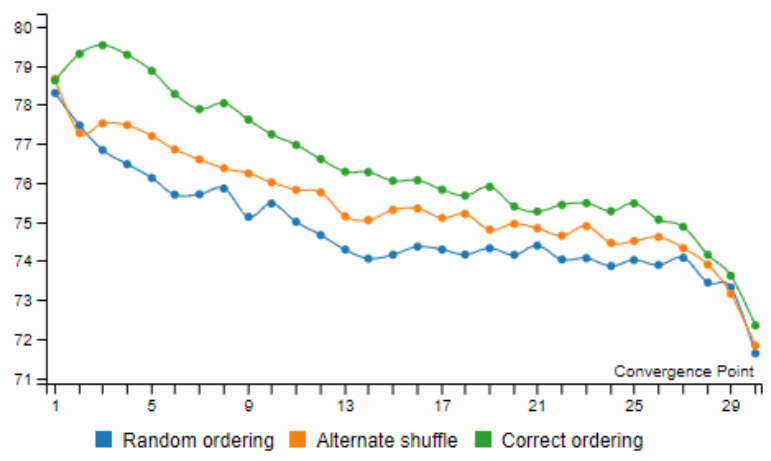
\includegraphics[width=0.6\linewidth]{img/cnnanalysis1.png}
\end{figure}

CNNs fail to fully incorporate sequential information -- performance on random ordering and correct ordering are marginally near each other

Performance with correct ordering on window size 7 $\approx$ random ordering on window size 1

	
\end{frame}


\begin{frame}{Analysis}
	
	\begin{figure}
		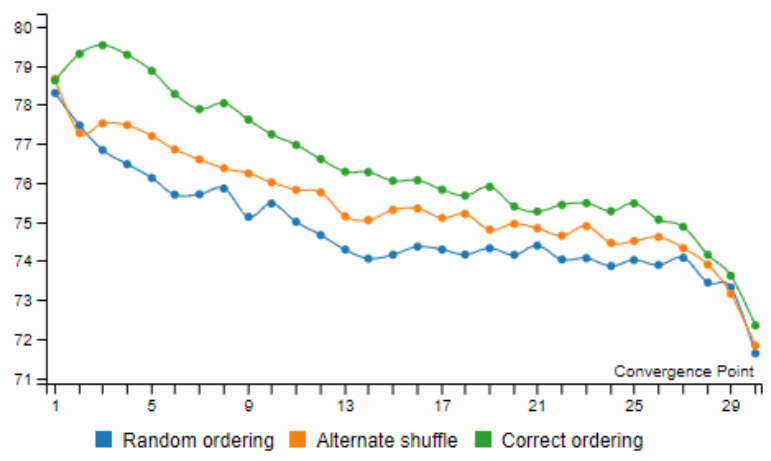
\includegraphics[width=0.5\linewidth]{img/cnnanalysis1.png}
	\end{figure}


Increasing window size $\to$ worse in capturing sequential information

But: Performance on random ordering is still higher than other context blind algorithms like bag-of-words

CNNs still learn something valuable! What?
	
\end{frame}


\begin{frame}{Experiment 2: What it learns}

Train a CNN with window size 1 on sentiment classification

- Convolution acts over a single word $\to$ no ability to capture sequential information
	
- Words will always have same respective convolution output

- Convolution layer here acts like an embedding transformation, where input embedding space is transformed into another space
	
	
\end{frame}


\begin{frame}{Analysis}
	
	\begin{figure}
	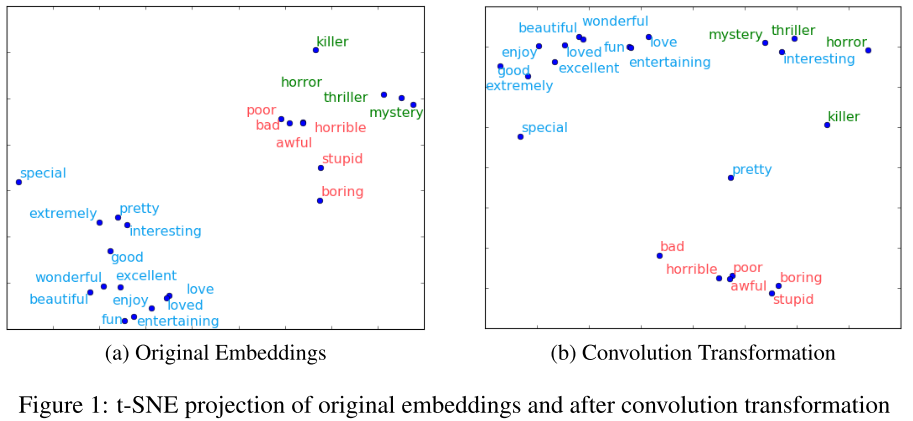
\includegraphics[width=1.0\linewidth]{img/cnnanalysis2.png}
\end{figure}


Blue = positive sentiment

Red = negative sentiment

Green = semantically close to negative sentiment words

\end{frame}


\begin{frame}{Analysis}
	
	\begin{figure}
		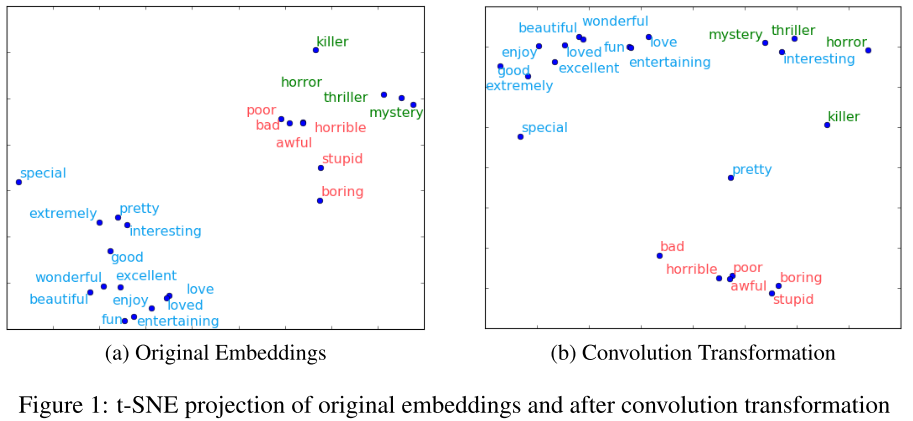
\includegraphics[width=1\linewidth]{img/cnnanalysis2.png}
	\end{figure}
	
	
Convolution layer tunes input embeddings $\to$ closer to the positive sentiment cluster than to their original semantic cluster


\end{frame}


\begin{frame}{Analysis}
	
	\begin{figure}
		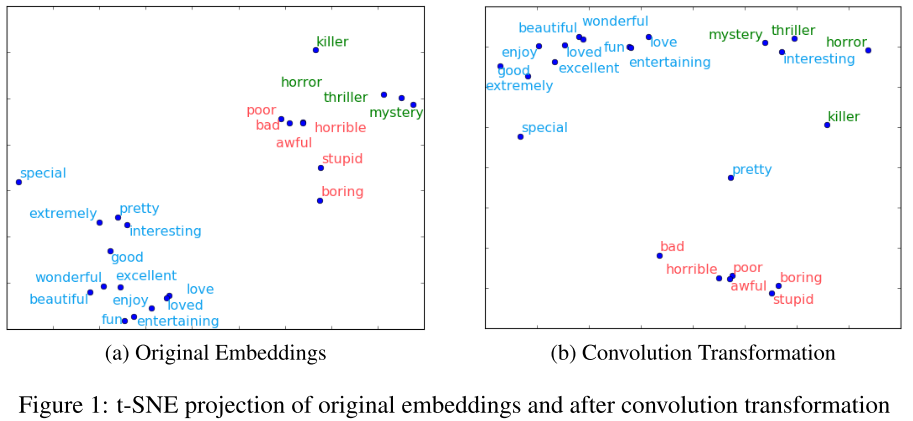
\includegraphics[width=1\linewidth]{img/cnnanalysis2.png}
	\end{figure}
	
	
\begin{small}
	
	“killer” in the original space very close to negative words “bad” and “awful” (Glove embeddings)
	
	However in the sentiment dataset, “killer” is often used to describe a movie very positively
\end{small}	
\end{frame}


\begin{frame}{Take-home message}
	
	
Single convolution filter output value captures a weighted summation over all the features of the original word embedding.

This enables the network to learn more task appropriate features as	many as the number of filters.

\bigskip

\fullcite{Madasu.AnveshRao.2019.EMNLP}
	
\end{frame}


\begin{frame}{Summary}





Convolutional networks can deal with variable sized input

- Sparse connectivity, parameter sharing
- Narrow vs wide convolution

Pooling enables focus on most relevant features

- Max-over-time pooling

Convolutional networks for NLP

- Sentence classification
	
\end{frame}


\begin{frame}{License and credits}
	
	\begin{columns}
		\begin{column}{0.7\textwidth}
			Licensed under Creative Commons Attribution-ShareAlike 4.0 International (CC BY-SA 4.0)
		\end{column}
		\begin{column}{0.2\textwidth}
			
\includegraphics[width=0.9\linewidth]{img/cc-by-sa-icon.pdf}
		\end{column}
	\end{columns}
	
	\bigskip
	
	Credits
	
	\begin{scriptsize}
		
		Ivan Habernal, Steffen Eger
		
		Content from ACL Anthology papers licensed under CC-BY \url{https://www.aclweb.org/anthology}
		
		Review screenshots courtesy of \url{https://www.rottentomatoes.com}
		
	\end{scriptsize}
	
\end{frame}

\begin{frame}[allowframebreaks]{References}
	\printbibliography
	%  \bibliography{bibliography}
	%  \bibliographystyle{abbrv}
\end{frame}

\end{document}

